\subsection{Umfrage Dashbaord}
\label{ssec:UmfrageDashboard}

Das Herzstück der Applikation soll das Erstellen einer Umfrage sein. 
Hier soll der Benutzer die Möglichkeit haben, eine Umfrage zu erstellen, die verschiedene Fragetypen beinhaltet. 
Fragetypen sind exemplarisch: 
%
\begin{itemize}
	\item Freitext (Single Input)
	\item Checkbox, Matrix (Multiple Choice)
	\item Radiogroup, Marix (Single Choice)
	\item Dropdown 
	\item Rating (Bewerung Skala)
	\item Boolean (Ja/Nein)
	\item Datepicker (Datumsfelder)
\end{itemize}
%
Der Benutzer soll einen Titel sowie eine Beschreibung seiner Umfrage definieren können. 
Darüber hinaus soll diese erstellte Umfrage als Vorlage \engl{Template} dienen, um basierend auf ihr verschiedene Umfragen erstellen zu können oder auch eine bestehende Umfrage erweitern zu können. 
Diese soll dann über einen neuen \emph{Sourveycode} realisiert werden. 

\abb \myRefGeneral{fig:SurveyCreatorImplement} stellt den Umfrageeditor der Anwendung dar, indem der Benutzer seine Umfragen erstellen sowie editieren kann. 
Die Umfragen sollen spezifisch nur für den angemeldeten Benutzer sichbar sein. 
Zudem soll der Benutzer noch die Möglichkeit haben, über eine Suchfunktion in seinen Umfragen nach einer geeigneten Umfrage zu suchen. \newline
Darüberhinaus soll dem Benutzer visuell dargestellt werden, wieviele Umfragen er basierend auf dieser Vorlage (Master Survey) erstellt hat. 
Des weiteren soll dem Benutzer ermöglicht werden, Umfragen, die noch nicht veröffentlich wurden, zu editieren und zu löschen. \newline
Über eine Button \enquote{Publish survey} soll der Benutzer eine Umfrage basierend auf dieser Master Survey erstellen können. 
Ihm soll visuell dargestellt werden, dass das Anlegen erfolgreich war und den generierten Sourveycode anzeigen. 
Diese wird seinem Result-Dashboard hinzugefügt (Kap. \myRefGeneral{ssec:ResultDashboardImplement}). 

\begin{figure}[hp]
	\centering
	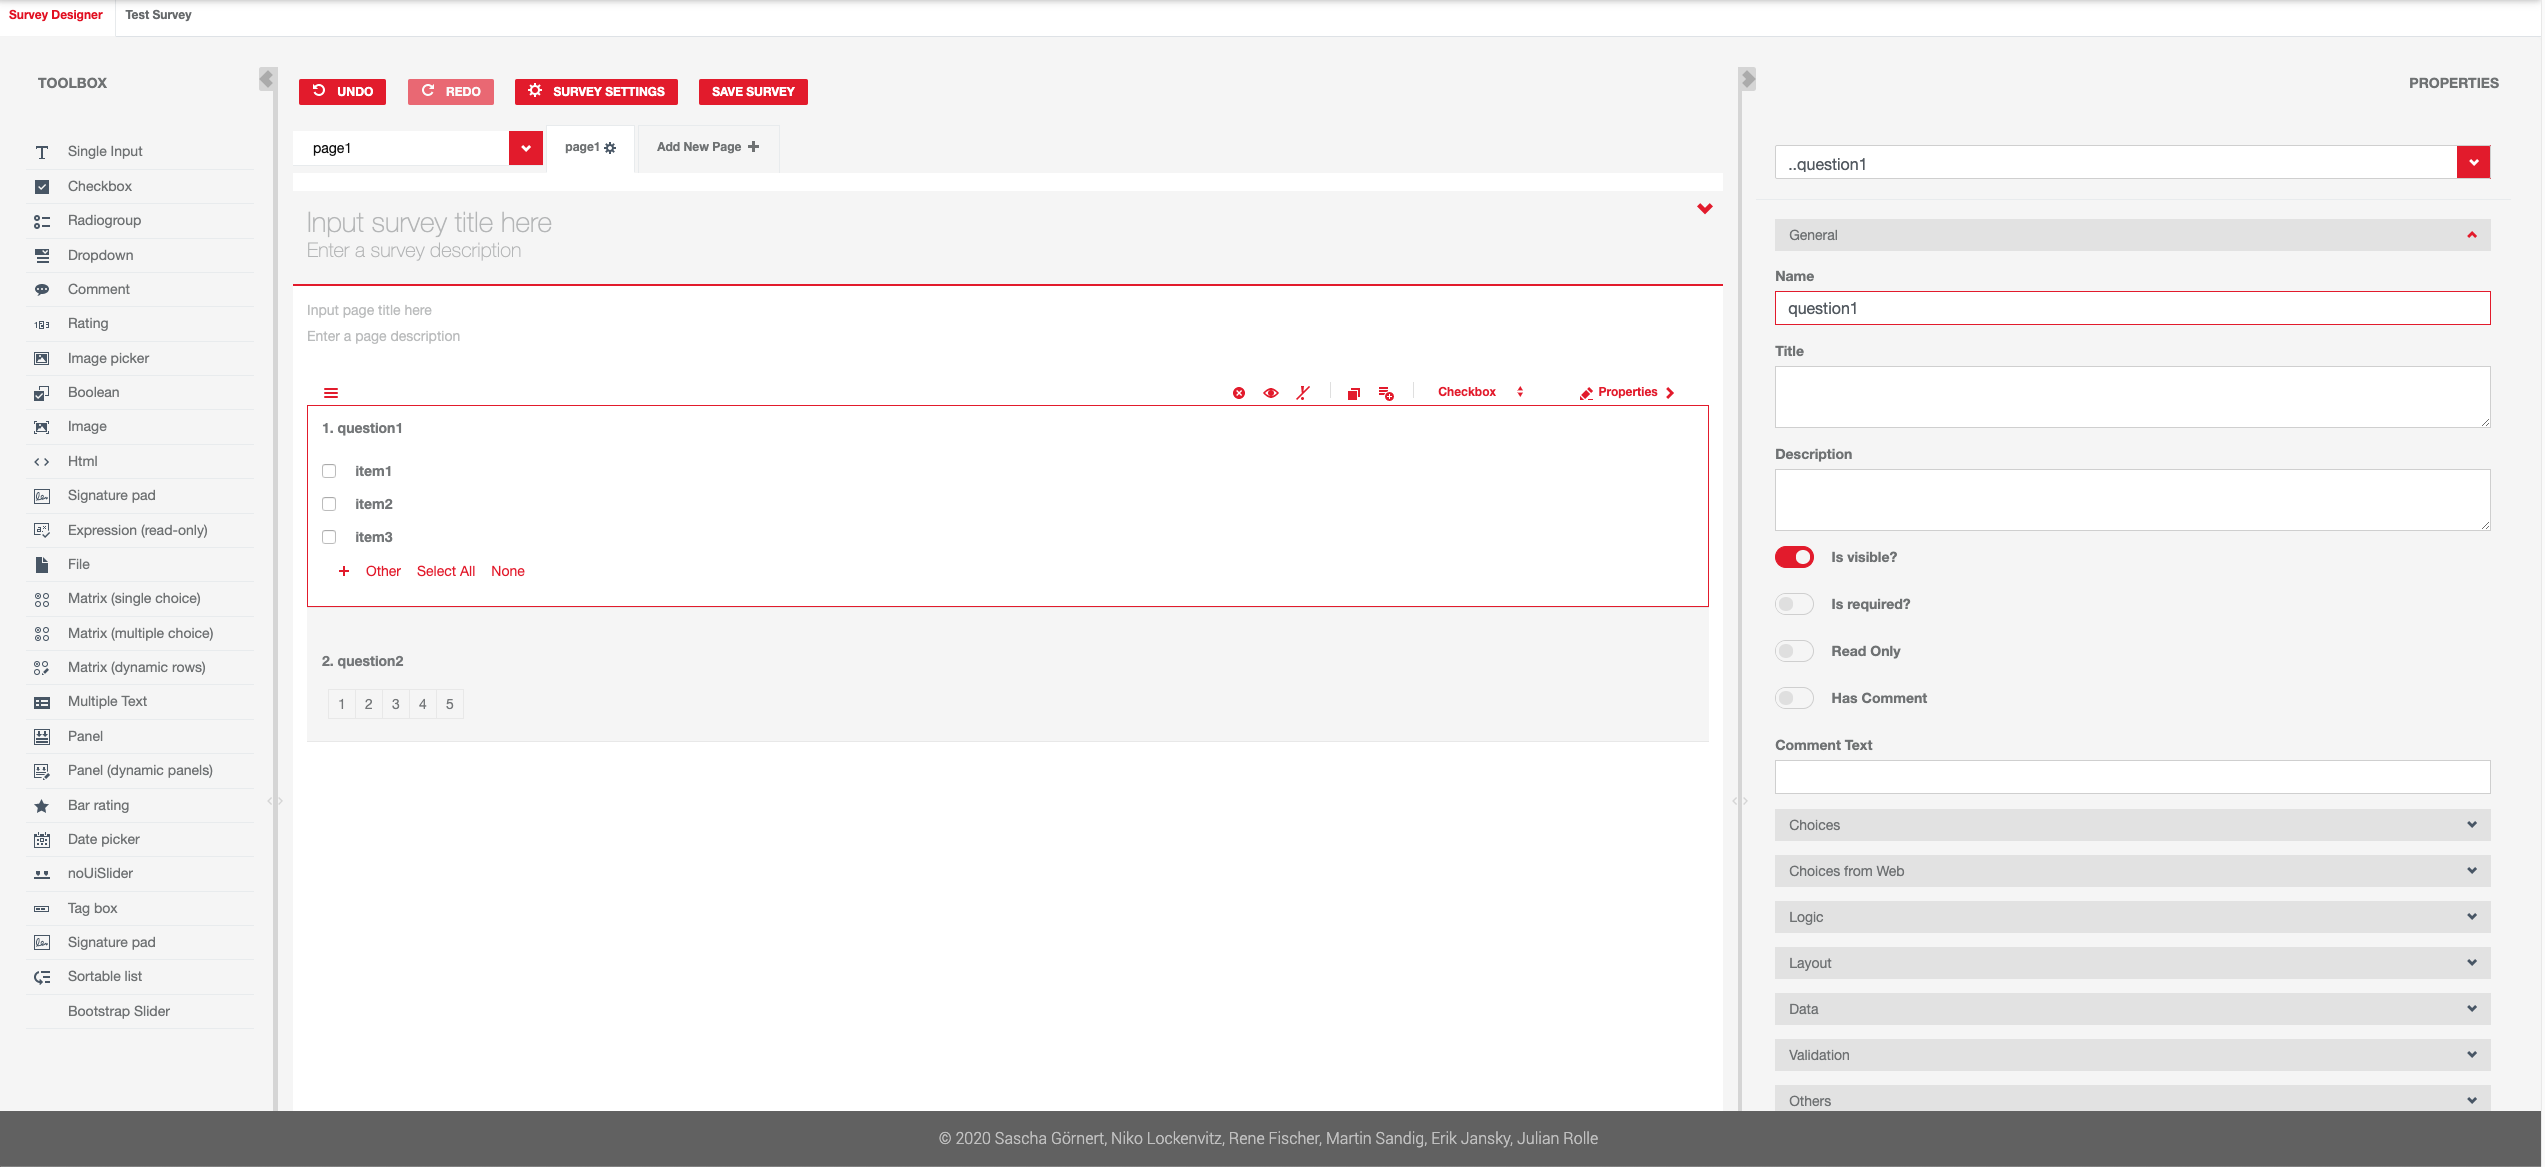
\includegraphics[width=0.95\textwidth, keepaspectratio]{img/client/CreateSurveyMaster.png}
	\captionsetup{justification=centering, format=plain}
	\caption[\acf{UI}: Erstellen einer Umfrage]{\acf{UI}: Erstellen einer Umfrage \\ \quelleScreenshot}
	\label{fig:SurveyCreatorImplement}
\end{figure}